% res_steady.tex -- Results 4.2: the steady payload error, rig and twin.
% Assembled 9 Oct (structure audit) from sim_results.tex (tracker initial condition, disturbance
% rejection, other approaches), controller.tex (the box's effect, the damping ratio), rig_results.tex
% (the ring sat low, tilt with height, the -x drift) and sim_robustness.tex (wrong model values; the
% attach case moved to Section 4.4). Tables by tools/thesis_sim_tables.py, figures by
% tools/thesis_sim_figures.py; run ids in configs/thesis_figures.yaml. Cells give the mean over repeats
% with the number of runs in brackets.
% Rig sources (from rig_results.tex): docs/rig_2026-09-30_review.md, rig_2026-09-30_replay.md,
% rig_2026-09-30_force_balance.md, registry RIG-0930-* and RIG-1001-* (h1, h2-z080, c1-z100, f8-z100,
% h5-z100-rot120, h6-z100-xp60), logs results/rig/2026-10-01/<flight>_logs; B4 offline replay
% (2026-10-01_load_ext_force.md); CURRENT_STATE 7 items 8 and 10 (16 and 23 Sep); twin R0817/R0818,
% R0834-R0839. The H6 drift is 2.8 cm in the registry and 4.5 cm in the 3 Oct review recompute:
% reported as 3-5.
% FIGURE TODO (thesis-figure skill): 1 Oct ring height vs time for H1/H2/C1/H5 with the cap and the
% integral; tilt vs ring height; plan view of the -x drift with the rotation test.

\subsection{Steady payload error}
\label{sec:res_steady}

What leaves a steady error in the payload's position, and what removes it? Each source below is set
against the same flight without its remedy: the tracker's relaxed initial condition, the breakaway cap
held for the whole flight, and no integral action for forces and wrong model values. The bar is the
ring back within 1\,cm of its target, the band used for the recovery times below.

\subsubsection{The tracker's initial condition}
\label{sec:res_ic}

An earlier version of the tracker relaxed its initial condition to a box with $\epsilon = 0.025$
(Section~\ref{sec:tracker}). Figure~\ref{fig:tracker_x0} and Table~\ref{tab:x0} compare this relaxed
initial condition with node~0 pinned to the measurement ($\epsilon = 0$), both without integral
action.

\begin{figure}[h]
\centering
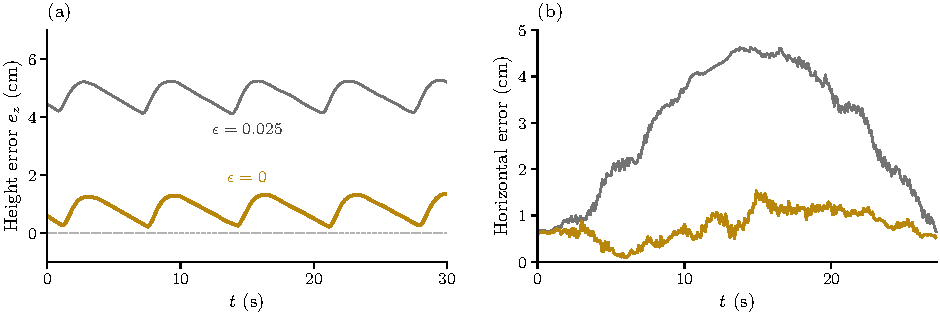
\includegraphics[width=\textwidth]{Images/tracker_x0.pdf}
\caption[Effect of the tracker's initial condition]{Effect of the tracker's initial condition without integral action: node~0 pinned to the
measured state ($\epsilon = 0$, gold) against the relaxed box ($\epsilon = 0.025$, grey). Gazebo rig
twin from a floor start, three UAVs. (a) Hover at 1.0\,m: ring height error from 10\,s after the
lift. Both settings show the same 1\,cm, 7\,s heave. (b) Circle of radius 0.5\,m at 0.125\,m/s:
horizontal ring error over the first lap including its 4\,s spin-up, sampled when the planner's
reference updates (10\,Hz). Dashed in (a): zero error. One run of each case is shown;
Table~\ref{tab:x0} gives the means.}
\label{fig:tracker_x0}
\end{figure}

\begin{table}[h]
\centering
\caption{Ring error with the relaxed and the pinned initial condition, no integral action. The
circle with $\epsilon = 0.025$ is a single run on an earlier code version; its horizontal error
reproduces on the current code (2.8\,cm, with the height integral on).}
\label{tab:x0}
% generated by tools/thesis_sim_tables.py
\begin{tabular}{llcc}
\toprule
Case & Metric & $\epsilon = 0.025$ & $\epsilon = 0$ \\
\midrule
Gazebo, hover at 1.0\,m & height error (cm) & +4.8 (2) & +0.9 (2) \\
Gazebo, circle & horizontal error, mean (cm) & 2.8 (1) & 0.8 (2) \\
 & height error (cm) & +4.8 (1) & +0.8 (2) \\
\bottomrule
\end{tabular}

\end{table}

With the box, each tracker could start its prediction from any state within 2.5\,\% of the
measured one, about 3.5\,cm of height at 1.4\,m, so the box acted as a dead band. The solver used that
freedom to treat its UAV as closer to the reference than it was, so small errors were not corrected:
the formation came to rest at the box's edge, and the payload held about 5\,cm above its target in
simulation. Pinning node~0 brings the offset to under 1\,cm without any integral action.
% --- original text, flown before the rig twin; kept to refill this place:
% rest at its edge, and the payload held 5--7\,cm above its target in simulation. With the box removed
% the offset disappears without any integral action.
The remainder is attributed to
the rods' 0.075\,kg mass, which the planner does not model: they hold 52$^\circ$ instead of the
planned 45$^\circ$. This is not yet tested with node~0 pinned. With the box in place, adding the
rods' mass to the planner's model corrected the rod elevation but did not move the height.

\redo{the relaxed box against node~0 pinned on a plant that matches the controller's model (the software-in-the-loop bench, once it flies the twin), three UAVs, hover: whether the box is the whole of the height offset, and whether the rods then hold the planned 45$^\circ$ and tension.}
% --- original text, flown before the rig twin; kept to refill this place:
% With the box, each tracker could start its prediction from any state within 2.5\,\% of the
% measured one. The solver used that freedom to treat its UAV as closer to the reference than it
% was, so small errors were not corrected. In SIL, where the plant matches the model, this was the
% whole of the payload's height offset. Pinning node~0 removes it, and the rods hold the planned
% 45$^\circ$ and the planned tension. In Gazebo the offset drops to under 1\,cm. The remainder is attributed to

The box was a fraction of each \emph{absolute} coordinate, so it widened as the UAVs moved away from
the world origin. The circle's error with the box grows with the ring's distance from the origin,
which is consistent with this (Figure~\ref{fig:tracker_x0}b), although on this circle the distance and
the phase of the lap change together. Pinning node~0 also removes most of that error.

The four-UAV circle and figure-8 of Table~\ref{tab:traj} were also flown with the relaxed box,
$\epsilon = 0.025$ (Figure~\ref{fig:traj}). Pinning node~0 cut the
horizontal error over the motion from 3.0 to 1.0\,cm on the circle and from 2.9 to 0.8\,cm on the
figure-8, and the height error from $+3.2$ to $-1.7$\,cm. The relaxed box's error grows as the ring
moves away from the world origin and shrinks as it returns, in both shapes.

\begin{figure}[h]
\centering
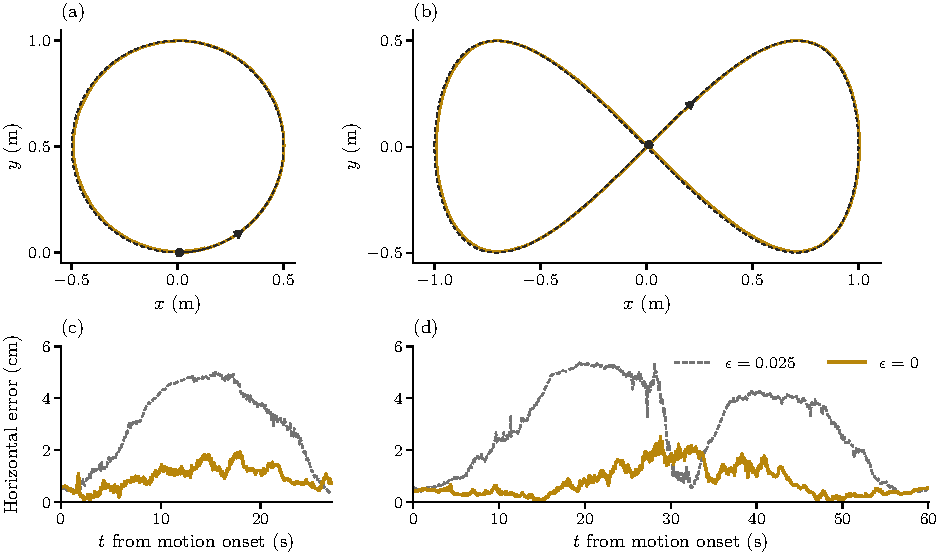
\includegraphics[width=\textwidth]{Images/trajectories.pdf}
\caption[Trajectory tracking with four UAVs]{Pinning node~0 cuts the four-UAV trajectory error by about
a factor of three. (a) Circle of radius 0.5\,m, one lap of 27\,s including a 4\,s spin-up; (b) a
2\,m\,$\times$\,1\,m figure-8 in 60\,s. Gold: ring path with $\epsilon = 0$; dark dashed: reference;
dot and arrow: start and direction. (c, d) Horizontal ring error from the onset of motion, sampled
when the planner's 10\,Hz reference updates, with $\epsilon = 0$ (gold) and the relaxed box
($\epsilon = 0.025$, dashed). Gazebo rig twin, four UAVs on the even ring, ring at 1.0\,m; one run of
each.}
\label{fig:traj}
\end{figure}

Landing is not yet resolved, with or without the box. In 21 Gazebo flights with $\epsilon = 0$, one
UAV tipped over during landing after the payload had touched down, as 2 of 32 earlier landings with the
box had. Both come from landing, not from the box, and the landing of Section~\ref{sec:sim_landing}
removes them.

\subsubsection{The breakaway cap}
\label{sec:res_cap}

On the rig on 1 October (Table~\ref{tab:rig_oct1}), without the height integral the ring held 5\,cm low at 0.5\,m, and at
higher targets it sat 20--30\,cm low before the integral took over, which then saturated at its bound.
The figure-eight, where the integral does not run, held the ring 29\,cm low. The shortfall was largest
on the flights whose ring broke free at the smallest fraction of the planned pull. The cause was
found afterwards in the logs: the breakaway freeze had held the pull at that fraction for the whole
flight, so the trackers were told the rods pull 7--27\,\% less than they do. Holding the pull at
75\,\% in the Gazebo twin reproduced both symptoms on the rig: the ring 23--26\,cm low and the rods
steepened from 52 to 58$^\circ$. Releasing the cap once the lift starts restored the twin's height
to the no-cap value (Section~\ref{sec:sim_to_real}). This fix has not yet been flown.

\subsubsection{External forces}
\label{sec:res_force}

A constant force was applied to the ring for 15\,s in hover: 0.6\,N downward, about the weight of a
60\,g object, and 0.4\,N horizontally. Both were sized so that the integral stays inside its
bound, at 56\,\% and 51\,\% of it. Without an integral the ring settles 8.4\,cm and 7.6\,cm away, which gives the closed loop's
stiffness to a force on the ring: $K_z = 7.1$\,N/m and $K_{xy} = 5.3$\,N/m, the values used for
$K$ in \eqref{eq:lumped_int}. Figure~\ref{fig:disturbance} shows the model integral on the horizontal push, and
Table~\ref{tab:disturbance} gives both pushes and compares it with the target-shift form.

\begin{figure}[h]
\centering
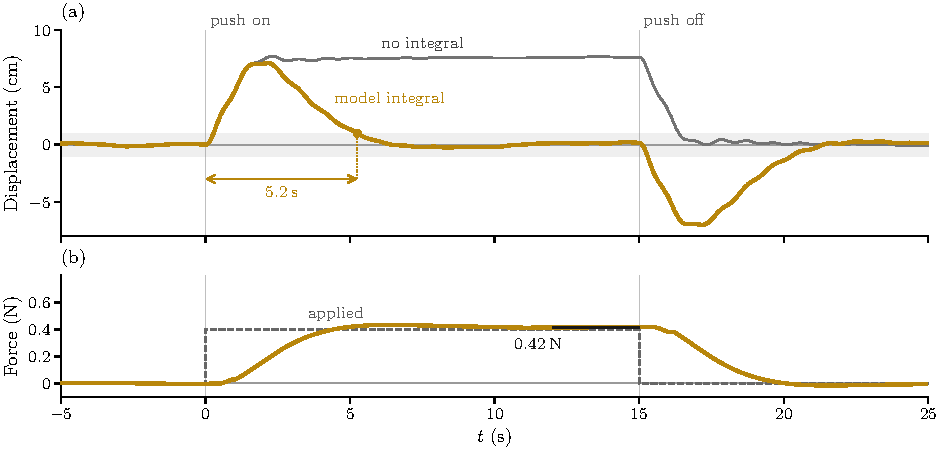
\includegraphics[width=\textwidth]{Images/disturbance.pdf}
\caption[Rejection of a constant force on the ring]{Rejection of a constant force on the ring, Gazebo rig twin, three UAVs, hover at 1.0\,m.
A 0.4\,N horizontal push acts from 0 to 15\,s. (a) Ring displacement along the push, relative to its
mean over the 5\,s before: no integral (grey) and the integral in the planner's model (gold). Band:
$\pm 1$\,cm. Arrow: time for the model integral to bring the ring back within 1\,cm for good. (b)
Change of the model integral's force $\mathbf{d}$ along the push from its value before the push
(gold), against the applied force (dashed). Black bar: its mean over the last 3\,s of the push. The
force holds still for about 0.7\,s after each step, while the ring moves faster than the integral's
5\,cm/s gate. One run of each case is shown; Table~\ref{tab:disturbance} gives the means and the
0.6\,N vertical push.}
\label{fig:disturbance}
\end{figure}

\begin{table}[h]
\centering
\caption{Disturbance rejection in the Gazebo rig twin with $\epsilon = 0$. One of the two
target-shift runs aborted on landing, after the push and its recovery; its push is included. The
change of the integral force is measured from its value before the push (0.06\,N vertically,
0.03\,N horizontally).}
\label{tab:disturbance}
% generated by tools/thesis_sim_tables.py
\small
\begin{tabular}{lccc}
\toprule
 & No integral & Target shift & Model integral \\
\midrule
\multicolumn{4}{l}{\emph{0.6\,N downward push on the ring}} \\
\quad steady displacement (cm) & 8.4 (2) & 0.3 (2) & 0.2 (2) \\
\quad peak displacement (cm) & 8.9 (2) & 6.6 (2) & 6.5 (2) \\
\quad overshoot on release (cm) & 0.4 (2) & 7.1 (2) & 7.0 (2) \\
\quad time to within 1\,cm after onset (s) & -- & 6.0 (2) & 6.1 (2) \\
\quad change of the integral force (N) & -- & -- & 0.58 (2) \\
\midrule
\multicolumn{4}{l}{\emph{0.4\,N horizontal push on the ring}} \\
\quad steady displacement (cm) & 7.6 (2) & n/a & 0.1 (2) \\
\quad peak displacement (cm) & 7.7 (2) & n/a & 7.2 (2) \\
\quad overshoot on release (cm) & 0.1 (2) & n/a & 7.0 (2) \\
\quad time to within 1\,cm after onset (s) & -- & n/a & 5.5 (2) \\
\quad change of the integral force (N) & -- & n/a & 0.42 (2) \\
\midrule
\multicolumn{4}{l}{\emph{One UAV producing more thrust than its map assumes}} \\
\quad height error (cm) & -- & 0.0 (2) & 0.0 (2) \\
\quad horizontal error (cm) & -- & 3.5 (2) & 0.0 (2) \\
\quad ring tilt (\si{\degree}) & -- & 6.4 (2) & 7.9 (2) \\
\bottomrule
\end{tabular}

\end{table}

Both forms of the integral bring the ring back to the target, and on the vertical push their
transients are the same to within a few per cent. With the conversion $K$ set to the measured
stiffness, the loop has the same gain whether the integral moves the target or enters the model. The
force the model integral learns is the force that was applied, within 3\,\% vertically and
4--5\,\% horizontally. Only the model form
acts horizontally, and it removes the horizontal push in the same way.

The integral reduces the peak only partly, by about a quarter vertically (8.9 to 6.5\,cm) and by
7\,\% horizontally (7.7 to 7.2\,cm), because it is slower than the cascade. The ring reaches most
of its uncompensated displacement within about 1\,s, while the integral's time constant is
$1/k_i = 2.5$\,s. When the push ends, the integral still holds the force it learned and drives the
ring past the target by about as much as the push displaced it at onset. This overshoot on release
is a property of integral action, not of where the integral acts. Table~\ref{tab:gain} shows the
trade-off. Doubling $k_i$ reduces the peak by 14\,\%, but the response rings and settles 55\,\% later,
the trend the damping relation of Section~\ref{sec:disturbance} predicts (with $\tau \approx 0.9$\,s,
measured vertically, and $k_i = 0.4$\,s$^{-1}$, $\zeta \approx 0.84$). This is a single run, and its
settling time is sensitive to the 1\,cm threshold against the 1\,cm heave of the hover. Keeping the
ring-speed gate only for the first 5\,s after the lift removes 7--8\,\% with no cost on this push; it has
not yet been flown on a trajectory, a hand-over or a landing.

\begin{table}[h]
\centering
\caption{Integral gain and gate on the 0.6\,N vertical push, model integral. Peak: largest
displacement during the push; overshoot and settling (to within 1\,cm): after it ends. Brackets:
number of runs.}
\label{tab:gain}
% generated by tools/thesis_sim_tables.py
\begin{tabularx}{\textwidth}{Xccc}
\toprule
Model integral & Peak (cm) & Overshoot (cm) & Settling (s) \\
\midrule
$k_i = 0.4$ & 6.5 (2) & 7.0 (2) & 4.7 (2) \\
$k_i = 0.8$ & 5.6 (1) & 6.0 (1) & 7.2 (1) \\
$k_i = 0.4$, speed gate only in the first 5\,s after the lift & 6.0 (1) & 6.4 (1) & 4.5 (1) \\
\bottomrule
\end{tabularx}

\end{table}

When one UAV produces more thrust than its map assumes, both forms hold the height. Only the model
form also removes the horizontal error, and the ring tilts 1.5$^\circ$ further. The thrust error is a
moment on the ring that neither form controls.

\redo{the two forms of the integral with the feedforward to the trackers scaled to 0.9, on a plant that matches the controller's model (the software-in-the-loop bench, once it flies the twin): the planned ring position half a second ahead against the actual one, the rod elevation, and how much of its bound the model integral uses.}
% --- original text, flown before the rig twin; kept to refill this place:
% In SIL the two forms can be compared directly, with the feedforward to the trackers scaled to 0.9.
% Both hold the target, but the reference-shift form raises the height target by 10\,cm and plans a
% climb towards it that never comes: the planned ring position half a second ahead is 4.2\,cm above
% where the ring is. The rods also settle at 48$^\circ$ rather than the planned 45$^\circ$. With the
% model integral the plan predicts what happens (0.0\,cm) and the rods hold 45$^\circ$. In SIL the model
% integral used 89\,\% of its vertical bound (0.95 of 1.07\,N) and raised its warning, because the
% conversion $K$ measured in Gazebo is lower than the SIL plant's stiffness.
% % TODO: generate the SIL plan-prediction numbers from the planner logs as the tables are.

\paragraph{The rig's pull towards $-x$.} In every rig flight of Table~\ref{tab:rig_oct1} the ring sat 3--17\,cm from its horizontal
reference, always towards the room's $-x$ direction, and nothing in the controller pulled it back.
The offset kept its direction when the whole system (ring and UAVs) was rotated by 124$^\circ$, so it
does not come from a particular UAV, rod or the ring. The force behind it was estimated offline from
the logs: the UAVs' delivered thrust, from the identified map and their measured attitudes, less the
total weight. Over the steady holds this gives a horizontal force of 0.41--0.52\,N towards $-x$,
about 1$^\circ$ of the fleet's thrust. At the planner's horizontal stiffness of about 5\,N/m that
explains offsets of 8--10\,cm. Moving the system 1.1\,m towards $+x$ reduced the offset to 3--5\,cm,
in a single flight. Two explanations remain open: a ground plane in the motion-capture calibration
tilted by about 1$^\circ$, which would put a component of gravity along $x$ in the frame the
controller works in, or air moving in the room. A plumb-line check of the calibration comes first at
the next session.

% sim_robustness.tex -- Results: robustness to wrong parameters (draft 4 Oct 2026).
% Sources: CURRENT_STATE 4.7 (E10, R0215-R0222, 10 Sep, attach demo, 0.6 kg ring), 4.8 (measure_rod_len,
% SIL R0308-R0327, 23 Sep, quadratic plant, notes 2026-09-23_geometry_autocal), 4.10 (kt_trim,
% R0405-R0432, notes 2026-09-23_kt_trim), decisions 2026-09-25 (height integral: R0557 0.661 vs
% R0558 0.600; pair 0.658 x2 vs 0.600 x3).
% All of these were flown with the tracker's node-0 box at 0.025 (default until 4 Oct), which is the
% +3.4 cm of the 0.634 baselines; the differences between arms are the result.
% T9 (tab:robust): R1038-R1067 (5 Oct, box 0, land fix), no-error baseline z_ki 0 R1013/R1023;
% generator tools/thesis_sim_tables.py table_robust.

\subsubsection{Wrong model values}
\label{sec:sim_robustness}

The controller is given the payload's mass, the rod lengths and the attachment radius, and each UAV's
thrust map. On the rig each of these is measured, and each can be wrong. This subsection collects the
tests of what a wrong value does.

\paragraph{The current controller.} Table~\ref{tab:robust} gives the rig twin's hover at 1.0\,m, three
UAVs from a floor start, with one wrong value in the controller while the simulated rig keeps the true
ones. Each case was flown without and with the height integral.
\begin{itemize}
    \item A wrong payload mass moves the hover by about 1.25\,cm per percent of mass, the same in
    both directions. The integral removes it while the miss is inside its 0.25\,m gate, with a target
    shift that mirrors the error. A 20\,\% overestimate puts the ring 2\,mm over the gate, so the
    integral never starts and the ring holds 26\,cm high: a miss beyond the gate is not taken for a
    static offset.
    % CHECK: "2 mm over the gate" against Table tab:robust (+25.8 cm against the 0.25 m gate, i.e. 8 mm);
    % the table is the mean over the hover, the gate may have seen a different instant.
    The bound matters as well: the 20\,\% underestimate needs 23\,cm of shift, which
    the earlier bound of 0.15\,m would have cut off, and the planner warns that the integral is near
    its bound.
    \item Measuring the rods at the hand-over absorbs a 5\,cm rod error completely. Without the
    measurement the ring sits 8\,cm high, and the integral does not help: a rod typed 5\,cm long
    measures as only partly taut, and the integral waits for every rod to be taut. For rods typed
    long, the measurement is therefore what makes the integral available; a rod typed short reads as
    taut, and that case was not flown.
    \item A 2\,cm error in the attachment radius has no visible effect.
\end{itemize}
The ring's tilt stayed within 1.0--1.3$^\circ$, slightly lower with the mass typed high, and all 28
flights landed.

\begin{table}[htbp]
\centering
\caption[Hover with a wrong model]{Hover at 1.0\,m with one wrong value in the controller's model,
Gazebo rig twin, three UAVs, $\epsilon = 0$, floor start. Each cell is the mean of two runs. Target
shift: the integral's correction to the height target at LAND. Tilt: mean over the four runs.
Landed: flights that landed without a tip. $^a$~The miss is over the integral's 0.25\,m gate, so the
integral never starts. $^b$~The unmeasured rods read as partly slack, so the integral's tautness
gate stays closed.}
\label{tab:robust}
% generated by tools/thesis_sim_tables.py
\begin{tabularx}{\textwidth}{>{\raggedright\arraybackslash}Xccccc}
\toprule
 & \multicolumn{2}{c}{Height error (cm)} & Target & & \\
\cmidrule(lr){2-3}
Error in the controller's model & no integral & integral & shift (cm) & Tilt (\si{\degree}) & Landed \\
\midrule
none & $+$0.9 & 0.0 & $-$0.8 & 1.2 & 4/4 \\
payload mass typed $+10$\,\% & $+$13.5 & 0.0 & $-$13.4 & 1.1 & 4/4 \\
payload mass typed $+20$\,\% & $+$25.8 & $+$25.8$^a$ & 0.0 & 1.0 & 4/4 \\
payload mass typed $-20$\,\% & $-$23.5 & 0.0 & $+$23.3 & 1.3 & 4/4 \\
rods typed $+5$\,cm, measured at the hand-over & $+$0.9 & $+$0.1 & $-$0.9 & 1.2 & 4/4 \\
rods typed $+5$\,cm, not measured & $+$8.2 & $+$8.2$^b$ & 0.0 & 1.1 & 4/4 \\
attachment radius typed $+2$\,cm & $+$0.9 & 0.0 & $-$0.9 & 1.2 & 4/4 \\
\bottomrule
\end{tabularx}

\end{table}

\paragraph{Rod length and attachment radius.}
\redo{hover with a wrong typed geometry, with and without the rod measurement at the hand-over, for the cases Table~\ref{tab:robust} does not have: rods typed short, the attachment radius typed 2\,cm short, and the combination (rods and radius wrong with the payload mass typed 20\,\% low).}
% --- original text, flown before the rig twin; kept to refill this place:
% \paragraph{Rod length and attachment radius.} The tautness gate scales each UAV's cable feedforward
% by its measured rod length over the typed one. A rod 4\,cm shorter than typed therefore reads as
% partly slack, the fleet flies about half of the cable feedforward, and the payload hangs 22\,cm low.
% Measuring the rods at the hand-over (Section~\ref{sec:takeoff}) removes this
% (Table~\ref{tab:rodlen}): rod errors of $\pm 4$\,cm and attachment-radius errors of $\pm 2$\,cm are
% absorbed to within 1\,cm, and with no error the measurement changes nothing. A mass error is not
% addressed by the measurement; with the payload 20\,\% heavier than typed the hover sat 9\,cm lower.
%
% \begin{table}[h]
% \centering
% \caption{Hover height with a wrong typed geometry, with and without measuring the rods
% (software-in-the-loop, target 0.60\,m, two runs each agreeing to 1\,mm).}
% \label{tab:rodlen}
% \begin{tabularx}{\textwidth}{>{\raggedright\arraybackslash}Xccc}
% \toprule
% Error & Measurement off & Measurement on & Measured rod \\
% \midrule
% none & 0.634 & 0.634 & 0.500 \\
% rod 0.46\,m, typed 0.50\,m & 0.416 & 0.631 & 0.460 \\
% rod 0.50\,m, typed 0.46\,m & 0.569 & 0.634 & 0.500 \\
% radius 0.27\,m, typed 0.25\,m & -- & 0.642 & 0.514 \\
% radius 0.23\,m, typed 0.25\,m & -- & 0.626 & 0.486 \\
% payload mass +20\,\% & -- & 0.540 & 0.500 \\
% rod $-4$\,cm, radius $-2$\,cm, mass +20\,\% & -- & 0.549 & 0.474 \\
% \bottomrule
% \end{tabularx}
% \end{table}

% CUT 5 Oct 2026 (legacy-only, not to be redone): the thrust-gain trim (kt_trim), a legacy-plant feature that is off on the rig and the twin.
% \paragraph{Thrust map.} A per-UAV estimate of the throttle-to-acceleration gain, computed from the
% UAV's own measured acceleration and its static share of the cable force, was built to correct a
% typed gain that is wrong. In the software-in-the-loop bench it brought the hover from 0.499 and
% 0.461\,m back to 0.614\,m with the gain typed 10 and 15\,\% high, with the estimates converging to
% within 1\,\% of the true gain, 3--9\,s after TAKEOFF and without overshoot. In Gazebo, from a floor start with the
% gain typed 10\,\% high, the fleet parked at 0.53\,m without it and lifted to 0.609\,m with it. It needed
% a floor-contact test, because while a UAV rests on the floor the floor carries part of its weight
% and the estimate read that as strong motors. With two UAVs it chattered at 2\,Hz until its inputs were
% time-aligned. On the rig the thrust map was instead identified directly (Section~\ref{sec:hardware}),
% and the estimate is kept off.

% CUT 5 Oct 2026 (legacy-only, not to be redone): the first height-integral test, superseded by Table tab:robust and the disturbance table.
% \paragraph{Height integral.} The bounded height integral on the target (Section~\ref{sec:disturbance})
% was first tested on a hover that sat high without it: 0.658\,m in two runs without the integral
% against 0.600\,m in three runs with it. In software-in-the-loop it held 0.600\,m in every static-offset
% case in both directions, stayed inert through the circle, and saturated with a warning when the error
% was a large gain fault rather than an offset.

\subsubsection{Estimators from the literature}
\label{sec:sim_methods}
% Sources: docs/overnight_2026-10-04.md (report table), registry R0841-R0955; notes 2026-10-03_*,
% 2026-10-04_* (offset_free_mpc = A, offset_free_innovation, indi_fext, kt_trim, pin_cable_rates,
% ancillary_tracker, l1_ring, xy_stiffness_b3); B4 notes 2026-10-01_load_ext_force (offline replay).
% All flown with the tracker box at 0.025 (before the x0 finding): the +4.8 cm hold is the box.

Before the initial-condition fix, the alternatives of Section~\ref{sec:disturbance} were tried
against the steady errors, each in the same three-UAV rig twin. Three cases represent the internal
errors: the hover itself, and one UAV whose thrust map is wrong in each direction (its real offset
0.03 above or below the 0.185 its tracker assumes). Two represent external forces: a 1\,N horizontal
push on the ring, and a 0.4\,m/s wind during the orbit. Table~\ref{tab:methods} in
Appendix~\ref{sec:app_negatives} gives the results and the details of each approach. All of them were
flown with the tracker's relaxed initial condition, so the hover without any correction sits 4.8\,cm
high; the comparisons between rows still hold. In short, the height integral on the target zeroes the
height in every case and does nothing horizontally; the force balance removes the push and most of
the wind but cannot see the internal height offset; the offset-free observer helps everywhere but
converges slowly; and the measured cable force is the only approach that levels the ring against one
UAV's wrong thrust map, but a UAV tipped in four of its six landings.

Two conclusions carried forward. First, the internal height offset was not a force at all, which is
why no force estimate could find it; it turned out to be the tracker's initial condition.
Second, a wrong thrust map on one UAV is a moment on the ring, and only a correction of that UAV's own
force removes the tilt it causes. A force on the ring, estimated or integrated, can only move the
whole formation.

\subsubsection{Tilt and height}
\label{sec:res_tilt}

On the rig the ring's tilt fell with its height. Over the first three flights of
Table~\ref{tab:rig_oct1} the ring's mean tilt fell from
5.0$^\circ$ at 0.45\,m to 2.5$^\circ$ at 0.67\,m and 1.6$^\circ$ at 0.94\,m; the later hovers at
0.9--1.0\,m had 2.2--3.8$^\circ$. Close to the floor the ring sits in the UAVs' downwash and its
recirculation off the floor, and flying higher was the most effective single change for a steady
ring.

\subsubsection{Sources of steady error}

Table~\ref{tab:error_sources} collects the sources found, how each shows at the payload and what
removes it.

\begin{table}[h]
\centering
\small
\caption{Sources of steady payload error found in this work, how each shows at the payload and what
removes it.}
\label{tab:error_sources}
\begin{tabularx}{\textwidth}{>{\raggedright\arraybackslash}p{3.2cm}>{\raggedright\arraybackslash}X>{\raggedright\arraybackslash}Xl}
\toprule
Source & Signature at the payload & Remedy & Section \\
\midrule
Tracker's relaxed initial condition & held high in hover; error grows with the distance from the world
origin; not a force, so no force estimate finds it & pin node~0 to the measurement & \ref{sec:res_ic} \\ \addlinespace
Breakaway cap held for the whole flight & held low; rods steeper than planned & release the cap once
the lift starts & \ref{sec:res_cap} \\ \addlinespace
External force (a push, wind, the rig's pull towards $-x$) & steady displacement along the force &
integral in the planner's model; force balance & \ref{sec:res_force} \\ \addlinespace
Wrong payload mass & height offset in proportion to the mass error & height integral, inside its gate
and bound & \ref{sec:sim_robustness} \\ \addlinespace
Rods typed long & held high; the rods read partly slack, so the integral's gate stays closed & measure
the rods at the hand-over & \ref{sec:sim_robustness} \\ \addlinespace
The rods' unmodelled mass & rods steeper than planned & integral action; the rod mass in the planner
corrects the elevation only & \ref{sec:res_ic} \\ \addlinespace
One UAV's thrust map wrong & ring tilt and a horizontal offset: a moment on the ring & a correction of
that UAV's own force (measured cable force) & \ref{sec:res_force}, \ref{sec:sim_methods} \\
\bottomrule
\end{tabularx}
\end{table}
